% conceptualisation of signature detection
    % small unit
    % complex descirption (F&F)
    % cluster analysis
The method of identification of spatial signatures consists of three top-level steps.
First, we delineate a spatial unit of analysis that reflects the structure of
urban phenomena on a very granular level. Then we characterise each of them
according to form and function, capturing the nature of each unit and its spatial
context. Finally, we use cluster analysis to derive a typology of our spatial units
that, once combined into contiguous areas, forms a typology of spatial signatures.

\subsection*{Spatial unit}
% spatial unit
    % conceptualisation of enclosed tessellation
    % rules
        % indivisible
        % internally consistent
        % geographically exhaustive
    % options
        % admin boundaries
        % arbitrary grids
        % morphological units
    % ET design
        % barriers
        % enclosures
        % anchors
        % ET cells
The first major methodological decision relates to the definition of the
spatial unit. An ideal candidate needs to reflect space in a granular manner, and we argue
it should fulfil three conditions. First, it should be \textit{indivisible},
meaning that any subdivision would result in a unit that is incapable of
capturing the nature of urban form and function. Second, it needs to be
\textit{internally consistent} - it should always reflect only a single signature type.
Last, it should be geographically \textit{exhaustive}, covering the entirety of the study
area.

Spatial units used in literature can be split into three groups. One is using
administrative boundaries like city regions\cite{angel2020}, wards or census output areas\cite{alexiou2016}, that are
convenient to obtain and can be easily linked to auxiliary data. However,
those rarely reflect the morphological composition of urban space and, in some cases, may
even “obscure morphologic reality”\cite{taubenbock2019new}. At the same time, most of them
are divisible, and larger units are not always internally consistent. Another group is based on
arbitrary uniform grids linked either to spatial indexing methods like
H3\cite{brodsky2018h3} or Ordnance Survey
National Grid, or to ancillary data of remote sensing or other origins like a
WorldPop grid\cite{jochem2021tools}. Grids however cannot be considered internally
consistent as
they do not consider the underlying structure of the landscape.
Finally, urban morphology studies tend to use morphological elements as
street segments\cite{araldi2019}, blocks\cite{gil2012},
buildings\cite{hamaina2012a} or plots\cite{bobkova2019} as units of analysis.
Some of those
could be seen as indivisible and internally consistent, but since they are largely based
on built-up fabric, they are not exhaustive. For example, in areas without any building or
street, there
is no spatial unit to work with. Plots could be theoretically considered as exhaustive,
consistent and indivisible, but there is no accepted conceptual definition and unified
geometric representation\cite{kropf2018}.

We are, therefore, proposing an application of an alternative spatial unit called \textit{enclosed
tessellation cell} (ETC), defined as "the portion of space that results
from growing a morphological tessellation within an enclosure delineated by a series
of natural or built barriers identified from the literature on urban form, function and
perception"\cite{dab_mf_2021a}.
% We should drop a reference to the conceptual paper here.
ETCs follow the morphological tradition in that it is
based on the physical elements of an environment but overcome the drawbacks of
conventionally used units. Its geometry is generated in the three steps illustrated in a
Figure \ref{fig:et_diagram}. First, a set of features representing physical barriers
subdividing space, in our case composed of the street network, railways, rivers and a
coastline, is combined, generating a layer of boundaries (\ref{fig:et_diagram} A).
These then partition space
into smaller enclosed geometries called \textit{enclosures} (\ref{fig:et_diagram} B),
which can be very granular
or very coarse depending on the geographic context. In dense city centres where a single
enclosure represents a single block is a high frequency of small enclosures. At the same time, in the
countryside, this approach leads to very few large enclosures as their delimiters are far away
from each other. Enclosures are then combined with building footprints (\ref{fig:et_diagram} B),
which act as
anchors in space and potentially subdivide enclosures into enclosed tessellation cells using the
morphological tessellation algorithm\cite{fleischmann2020} (\ref{fig:et_diagram} D),
a polygon-based adaptation of Voronoi
tessellation. The resulting geometries are indivisible as they contain, at most, a single
anchor building, internally consistent due to their granularity and link to morphological
elements composing urban fabric, and geographically exhaustive as they cover an entire area
limited by specified boundaries.

\begin{figure}
    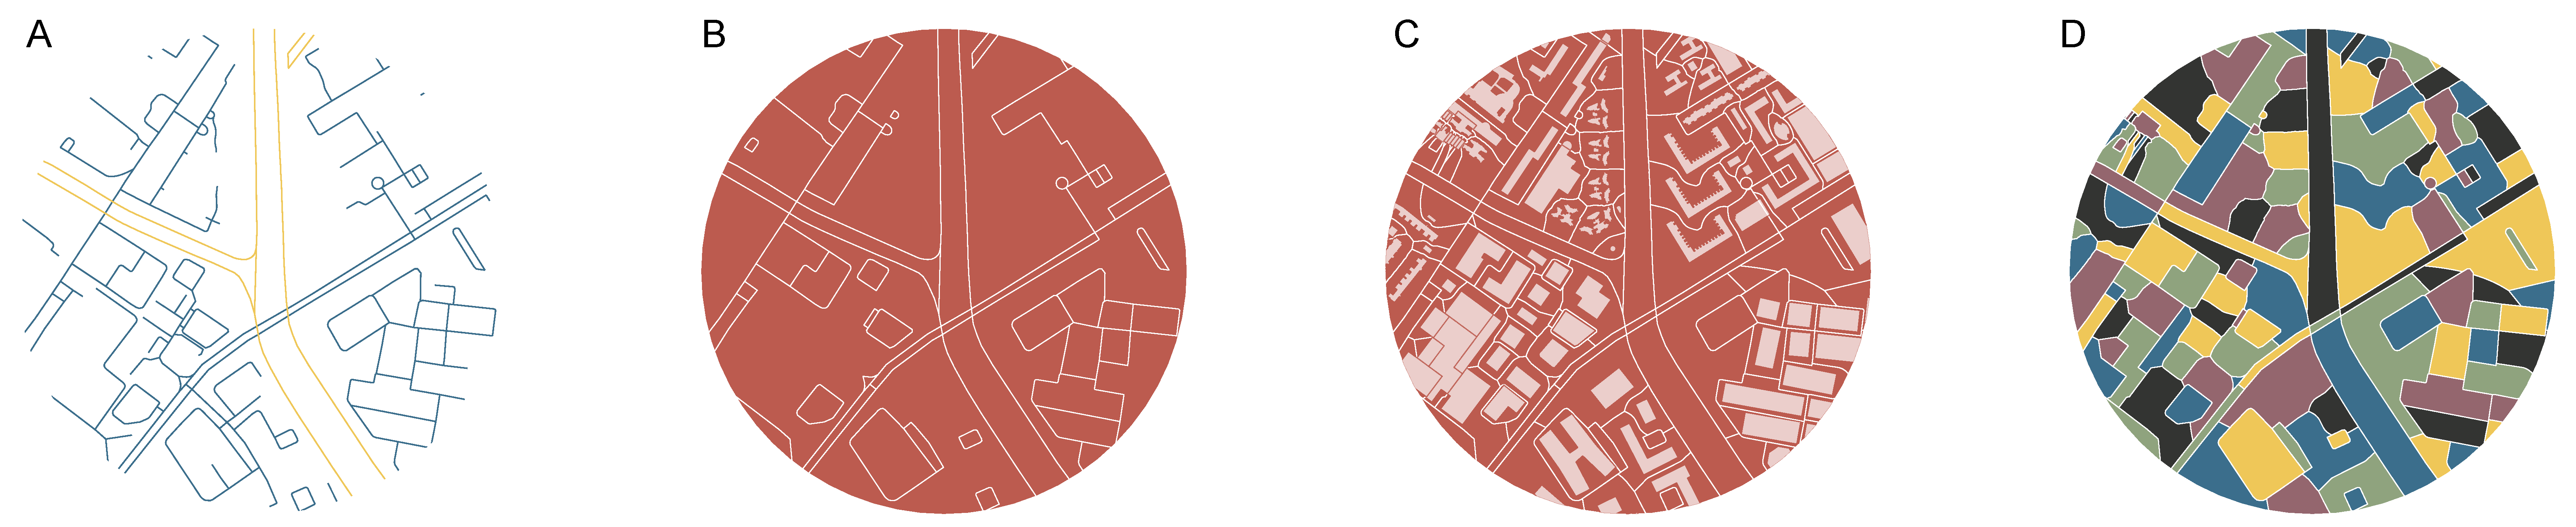
\includegraphics[width=\linewidth]{fig/et_diagram.pdf}
    \caption{Diagram illustrating the sequential steps leading to the delineation of
    enclosed tessellation. From a series of enclosing components, where blue are streets
    and yellow river banks (A), to enclosures (B), incorporation of buildings as anchors
    (C) to final tessellation cells (D).}
    \label{fig:et_diagram}
\end{figure}

    % data input
        % barries
            % roads from OS Open Roads
                % data description (simplified centerlines)
            % railway from OS OpenMap - Local
                % data description (simplified centerlines)
            % rivers from OS OpenRivers
                % data description (simplified centerlines)
            % coastline from OS Strategi®
                % data description (continuous enclosing geometry)
        % buildings
            % OS OpenMap - Local
            % data quality description (merged adjacent geometries)

In our ODP for Great Britain, street networks are extracted from OS
Open Roads datasets\cite{openroads2020} representing simplified road centrelines
cleaned of underground road segments.
Railways are retrieved from OS OpenMap - Local\cite{openmap2020}
("RailwayTrack" layer) which captures surface railway tracks. Rivers are extracted from
OS OpenRivers\cite{openrivers2020} representing river network of GB as centrelines, and a coastline is
retrieved from OS Strategi®\cite{strategi2016}, capturing coastline as a continuous line
geometry. Building geometry is extracted, again, from OS OpenMap - Local ("Building"
layer) and represents generalised building footprint polygons.\footnote{Note that the dataset
does not distinguish between individual buildings when they are adjacent (e.g. perimeter
block composed of multiple buildings is represented by a single polygon).}

% characterisation of space
\subsection*{Characterisation of space}
Spatial signatures capture the character of the built and unbuilt environment
based on two components - form and function. Each of them is quantified at the level of
individual ETCs using methods appropriate for each specific dataset. While form
is described using urban morphometrics (i.e. quantitative analysis of urban
form)\cite{dibble2019origin}, function is a composite of a variety of data inputs. We outline each
component with a bit more detail below.

\subsubsection*{Form}
    % form
        % input data
            % ET cells
            % bulidings
            % street network
        % morphometrics
            % different categories of characters
                % dimension
                % shape
                % spatial distribution
                % intensity
                % connectivity
                % diversity
            % different scales
                % individual elements -> adjacency -> networks
        % contextualisation
            % interest in characterisation of spatial patterns
            % distance-weighted higher order contiguity spatial weights
            % reflection of a statistical distribution of data within context
                % proxy of diversity
Morphometric characterisation of urban form is based on the numerical description
of four elements capturing the built environment - buildings, streets, ETCs, and
enclosures - and reflects their patterns based on six categories of
characters: dimensions, shapes, spatial
distribution, intensity, connectivity and diversity\cite{fleischmann2020a}. Each element is considered across
different scales, from the measurement of individual geometries, to relations of
neighbouring geometries, to a graph-based analysis of the street network. The combination of
elements, categories and scales results in a set of 59 individual morphometric
characters listed in the table \ref{tab:form}. The selection builds on the principles
outlined by \cite{dibble2019origin} and later explored by \cite{fleischmann2021}, both
following the rules derived by \cite{sneath1973numerical}. The gist is to include as
many characters present in literature as is feasible, while minimising potential
collinearity and limiting redundancy of information.


\begin{table}
\begin{tabular}{lll}
\toprule
                                            character &     category &               reference \\
\midrule
                                    area of building &    dimension &    \cite{hallowell2013} \\
                                perimeter of building &    dimension & \cite{vanderhaegen2017} \\
                        courtyard area of building &    dimension &     \cite{schirmer2015} \\
                    circular compactness of building &        shape &       \cite{dibble2019origin} \\
                                corners of building &        shape &    \cite{steiniger2008} \\
                            squareness of building &        shape &    \cite{steiniger2008} \\
            equivalent rectangular index of building &        shape &    \cite{basaraner2017} \\
                            elongation of building &        shape &    \cite{steiniger2008} \\
    centroid - corner distance deviation of building &        shape &  \cite{fleischmann2021} \\
        centroid - corner mean distance of building &    dimension &     \cite{schirmer2015} \\
                            orientation of building & distribution &     \cite{schirmer2015} \\
                        street alignment of building & distribution &     \cite{schirmer2015} \\
                        cell alignment of building & distribution &  \cite{fleischmann2021} \\
                        longest axis length of ETC &    dimension &  \cite{fleischmann2021} \\
                                        area of ETC &    dimension &     \cite{hamaina2012a} \\
                        circular compactness of ETC &        shape &  \cite{fleischmann2021} \\
                equivalent rectangular index of ETC &        shape &  \cite{fleischmann2021} \\
                                orientation of ETC & distribution &  \cite{fleischmann2021} \\
                            covered area ratio of ETC &    intensity &      \cite{hamaina2013} \\
                            length of street segment &    dimension &          \cite{gil2012} \\
                            width of street profile &    dimension &       \cite{araldi2019} \\
                        openness of street profile & distribution &       \cite{araldi2019} \\
                    width deviation of street profile &    diversity &       \cite{araldi2019} \\
                        linearity of street segment &        shape &       \cite{araldi2019} \\
                area covered by edge-attached ETCs &    dimension &  \cite{fleischmann2021} \\
                buildings per meter of street segment &    intensity &  \cite{fleischmann2021} \\
                area covered by node-attached ETCs &    dimension &  \cite{fleischmann2021} \\
                alignment of neighbouring buildings & distribution &       \cite{hijazi2016} \\
        mean distance between neighbouring buildings & distribution &       \cite{hijazi2016} \\
                perimeter-weighted neighbours of ETC & distribution &  \cite{fleischmann2021} \\
                area covered by neighbouring cells &    dimension &  \cite{fleischmann2021} \\
                reached ETCs by neighbouring segments &    intensity &  \cite{fleischmann2021} \\
                reached area by neighbouring segments &    dimension &  \cite{fleischmann2021} \\
                            node degree of junction & distribution &       \cite{boeing2018} \\
mean distance to neighbouring nodes of street n... &    dimension &  \cite{fleischmann2021} \\
                        mean inter-building distance & distribution &       \cite{caruso2017} \\
                weighted reached enclosures of ETC &    intensity &  \cite{fleischmann2021} \\
            reached ETCs by tessellation contiguity &    intensity &  \cite{fleischmann2021} \\
            reached area by tessellation contiguity &    dimension &  \cite{fleischmann2021} \\
                                    area of enclosure &    dimension &       \cite{dibble2019origin} \\
                            perimeter of enclosure &    dimension &          \cite{gil2012} \\
                    circular compactness of enclosure &        shape &     \cite{schirmer2015} \\
            equivalent rectangular index of enclosure &        shape &    \cite{basaraner2017} \\
            compactness-weighted axis of enclosure &        shape &   \cite{feliciotti2018} \\
                            orientation of enclosure & distribution &          \cite{gil2012} \\
        perimeter-weighted neighbours of enclosure & distribution &  \cite{fleischmann2021} \\
                    area-weighted ETCs of enclosure &    intensity &  \cite{fleischmann2021} \\
                local meshedness of street network & connectivity &   \cite{feliciotti2018} \\
                mean segment length within 3 steps &    dimension &  \cite{fleischmann2021} \\
            local cul-de-sac length of street network &    dimension &  \cite{fleischmann2021} \\
                reached area by local street network &    dimension &  \cite{fleischmann2021} \\
                reached ETCs by local street network &    intensity &  \cite{fleischmann2021} \\
                local node density of street network &    intensity &  \cite{fleischmann2021} \\
    local proportion of cul-de-sacs of street network & connectivity &        \cite{lowry2014} \\
local proportion of 3-way intersections of stre... & connectivity &       \cite{boeing2018} \\
local proportion of 4-way intersections of stre... & connectivity &       \cite{boeing2018} \\
local degree weighted node density of street ne... &    intensity &       \cite{dibble2019origin} \\
                    local closeness of street network & connectivity &        \cite{porta2006} \\
                square clustering of street network & connectivity &  \cite{fleischmann2021} \\
\bottomrule
\end{tabular}
\caption{\label{tab:form}Morphometric characters used to
describe the form component of spatial signatures. For details of the implementation,
refer to the reproducible Jupyter notebooks available at urbangrammarai.xyz.}
\end{table}

% Q: do we want to include some morphometric theory here? I'd say no since this is a
% data descriptor but I can add some if needed.

However, measuring individual characters is not enough to understand the predominant
spatial patterns. For some types of urban environment, high heterogeneity is not
uncommon. This means that using, for example, areas of building footprints would, in most cases, result
in largely discontinuous clusters that do not capture the pattern within an area. Therefore, we represent each of the
morphometric characters using three summary variables reflecting statistical distributions
of measured data within a spatial context of each ETC. Context is defined as
tenth
order of contiguity computed across the mesh composed of contiguous ETCs as illustrated
in figure \ref{fig:context}. Furthermore, each
value is weighted by the inverse distance between so-called poles of inaccessibility
(defined as a centre of a maximum inscribed circle) of each ETC. Three proxy variables
then capture the first, the second and the third quartile of the resulting weighted
distribution. Such a characterisation can capture the contextual tendency of each
morphometric character and hence identify contiguous clusters in both homogenous and
heterogeneous urban tissues. These contextual values are then used as an input for
cluster analysis while the original non-contextualised versions are left out, making the
final form component composed of 177 contextual characters.

\begin{figure}
    \centering
    \includegraphics[width=.8\linewidth]{fig/cell_context.png}
    \caption{Illustration of a definition of spatial context used to capture the
    distribution of values around each ET cell. For the yellow ET cell in the middle,
    we propose to define a neighbourhood of 10 topological steps on the tessellation
    and weight the importance of each cell within such an area by inverse distance
    between poles of inaccessibility of each cell.}
    \label{fig:context}
\end{figure}


\subsubsection*{Function}
    % function
        % input data
            % overview - from population and POIs to NDVI and night lights
            % include table with transfer methods
        % transfer methods overview
            % blg-based interpolation
            % areal interpolation
            % accessibility
            % euclidean distance
            % zonal statistics
        % contextualisation
            % depending on the transfer method, function-based characters we
            %  contextualised using the same method used in morphometrics
Characterisation of the function component uses a different approach. While data
describing urban form are not generally available in a processed format, forcing us to employ morphometric approaches, different aspects of function are often available as
open data products. 
%
We guide the compilation of functional characters following three main
principles: first, we identify from the literature on urban function key areas
to be represented; second, we translate those abstract areas into measurable
features; and third, we select open data available in for Great Britain that
allows for the redistribution of derivative products. 
%
With a list of function characters selected, the main goal of our characterisation of ETCs based on
function is to develop appropriate transfer methods to link data published as grids or
linked to administrative boundaries to ETCs.

In this work, we are using five different transfer methods: Areal interpolation,
Building-based dasymetric areal interpolation\cite{eli_knaap_2021_5047613} using building footprint area, Network-constrained accessibility,
Euclidean accessibility, and Zonal statistics. Areal interpolation is used when the
functional data covers the entirety of space in the
form of polygon geometry and when there is no assumption that the phenomena it captures
are linked directly to the human population, such as land cover data. When there is
an assumption of relation to the population, building-based dasymetric areal
interpolation is used instead. The main difference is that instead of ETC polygons,
building footprint polygons linked to individual ETCs are used as a target of
interpolation. That ensures that data like population estimates are linked to ETCs
proportionally to their ability to house population rather than by their area.
Network-constrained accessibility is used when the input data represents points of
interest like locations of supermarkets. Points are then snapped to the nearest node on
the street network and linked to the ETCs through the count of observations
accessible from the cell within 15 minutes of walk (1200m on the street network) and a distance to the nearest point. In
some cases, Euclidean (as-crow-flies) accessibility is measured instead to accommodate
for phenomena that are often outside the reach of a drivable network like water bodies.
Zonal statistics are used to transfer data originally stored in a raster
format to ETCs as the mean value of raster pixels intersecting each polygon
geometry. Finally, characters based on interpolation and zonal statistics are expressed
using their contextual versions following the method used for form characters to, again,
reflect the contextual pattern of measured values. As in the case of morphometric characters,
only contextual versions are then used in the cluster analysis. The selection of datasets and the chosen
transfer method are listed in the table \ref{tab:function}.

\begin{table}
    \begin{tabular}{lllll}
        \toprule
                                                                                                  character &                               data  &                                                                     source  &                    input geometry  &                                transfer method  \\
        \midrule
                                                                                                 Population &               Population estimates  &           ONS Census Output Area population estimates, Statistics.gov.scot  &      Vector (output area polygon)  &  Building-based dasymetric areal interpolation  \\
                                                                                               Night lights &                       Night Lights  &                                                 VIIRS DNB Nighttime Lights  &                     Raster (500m)  &                               Zonal statistics  \\
                                                       Workplace population [Agriculture, energy and water] &               Workplace population  &    ONS Census Workplace population, Scotland's census Workplace population  &      Vector (output area polygon)  &  Building-based dasymetric areal interpolation  \\
                                                                       Workplace population [Manufacturing] &               Workplace population  &    ONS Census Workplace population, Scotland's census Workplace population  &      Vector (output area polygon)  &  Building-based dasymetric areal interpolation  \\
                                                                        Workplace population [Construction] &               Workplace population  &    ONS Census Workplace population, Scotland's census Workplace population  &      Vector (output area polygon)  &  Building-based dasymetric areal interpolation  \\
                                                Workplace population [Distribution, hotels and restaurants] &               Workplace population  &    ONS Census Workplace population, Scotland's census Workplace population  &      Vector (output area polygon)  &  Building-based dasymetric areal interpolation  \\
                                                         Workplace population [Transport and communication] &               Workplace population  &    ONS Census Workplace population, Scotland's census Workplace population  &      Vector (output area polygon)  &  Building-based dasymetric areal interpolation  \\
                  Workplace population [Financial, real estate, professional and administrative activities] &               Workplace population  &    ONS Census Workplace population, Scotland's census Workplace population  &      Vector (output area polygon)  &  Building-based dasymetric areal interpolation  \\
                                         Workplace population [Public administration, education and health] &               Workplace population  &    ONS Census Workplace population, Scotland's census Workplace population  &      Vector (output area polygon)  &  Building-based dasymetric areal interpolation  \\
                                                                               Workplace population [Other] &                  Corine land cover  &                                         Copernicus Land Monitoring Service  &  Vector (land cover zone polygon)  &                            Areal interpolation  \\
                                                                                      Land cover [Airports] &                  Corine land cover  &                                         Copernicus Land Monitoring Service  &  Vector (land cover zone polygon)  &                            Areal interpolation  \\
                                                                     Land cover [Non-irrigated arable land] &                  Corine land cover  &                                         Copernicus Land Monitoring Service  &  Vector (land cover zone polygon)  &                            Areal interpolation  \\
                                                                Land cover [Industrial or commercial units] &                  Corine land cover  &                                         Copernicus Land Monitoring Service  &  Vector (land cover zone polygon)  &                            Areal interpolation  \\
                                                                                  Land cover [Salt marshes] &                  Corine land cover  &                                         Copernicus Land Monitoring Service  &  Vector (land cover zone polygon)  &                            Areal interpolation  \\
                                                                                     Land cover [Estuaries] &                  Corine land cover  &                                         Copernicus Land Monitoring Service  &  Vector (land cover zone polygon)  &                            Areal interpolation  \\
                                                                  Land cover [Sport and leisure facilities] &                  Corine land cover  &                                         Copernicus Land Monitoring Service  &  Vector (land cover zone polygon)  &                            Areal interpolation  \\
                                                                             Land cover [Green urban areas] &                  Corine land cover  &                                         Copernicus Land Monitoring Service  &  Vector (land cover zone polygon)  &                            Areal interpolation  \\
                                                                    Land cover [Discontinuous urban fabric] &                  Corine land cover  &                                         Copernicus Land Monitoring Service  &  Vector (land cover zone polygon)  &                            Areal interpolation  \\
                                                                                      Land cover [Pastures] &                  Corine land cover  &                                         Copernicus Land Monitoring Service  &  Vector (land cover zone polygon)  &                            Areal interpolation  \\
                                                                           Land cover [Broad-leaved forest] &                  Corine land cover  &                                         Copernicus Land Monitoring Service  &  Vector (land cover zone polygon)  &                            Areal interpolation  \\
                                                                      Land cover [Mineral extraction sites] &                  Corine land cover  &                                         Copernicus Land Monitoring Service  &  Vector (land cover zone polygon)  &                            Areal interpolation  \\
                                                                                    Land cover [Port areas] &                  Corine land cover  &                                         Copernicus Land Monitoring Service  &  Vector (land cover zone polygon)  &                            Areal interpolation  \\
                                                    Land cover [Road and rail networks and associated land] &                  Corine land cover  &                                         Copernicus Land Monitoring Service  &  Vector (land cover zone polygon)  &                            Areal interpolation  \\
                                                                                  Land cover [Water bodies] &                  Corine land cover  &                                         Copernicus Land Monitoring Service  &  Vector (land cover zone polygon)  &                            Areal interpolation  \\
        Land cover [Land principally occupied by agriculture, with significant areas of natural vegetation] &                  Corine land cover  &                                         Copernicus Land Monitoring Service  &  Vector (land cover zone polygon)  &                            Areal interpolation  \\
                                                                                  Land cover [Mixed forest] &                  Corine land cover  &                                         Copernicus Land Monitoring Service  &  Vector (land cover zone polygon)  &                            Areal interpolation  \\
                                                                                     Land cover [Peat bogs] &                  Corine land cover  &                                         Copernicus Land Monitoring Service  &  Vector (land cover zone polygon)  &                            Areal interpolation  \\
                                                                            Land cover [Natural grasslands] &                  Corine land cover  &                                         Copernicus Land Monitoring Service  &  Vector (land cover zone polygon)  &                            Areal interpolation  \\
                                                                           Land cover [Moors and heathland] &                  Corine land cover  &                                         Copernicus Land Monitoring Service  &  Vector (land cover zone polygon)  &                            Areal interpolation  \\
                                                                   Land cover [Transitional woodland-shrub] &                  Corine land cover  &                                         Copernicus Land Monitoring Service  &  Vector (land cover zone polygon)  &                            Areal interpolation  \\
                                                                       Land cover [Continuous urban fabric] &                  Corine land cover  &                                         Copernicus Land Monitoring Service  &  Vector (land cover zone polygon)  &                            Areal interpolation  \\
                                                                              Land cover [Intertidal flats] &                  Corine land cover  &                                         Copernicus Land Monitoring Service  &  Vector (land cover zone polygon)  &                            Areal interpolation  \\
                                                                                 Land cover [Sea and ocean] &                  Corine land cover  &                                         Copernicus Land Monitoring Service  &  Vector (land cover zone polygon)  &                            Areal interpolation  \\
                                                                             Land cover [Coniferous forest] &                  Corine land cover  &                                         Copernicus Land Monitoring Service  &  Vector (land cover zone polygon)  &                            Areal interpolation  \\
                                                                            Land cover [Construction sites] &                  Corine land cover  &                                         Copernicus Land Monitoring Service  &  Vector (land cover zone polygon)  &                            Areal interpolation  \\
                                                                      Land cover [Sparsely vegetated areas] &                  Corine land cover  &                                         Copernicus Land Monitoring Service  &  Vector (land cover zone polygon)  &                            Areal interpolation  \\
                                                                                    Land cover [Bare rocks] &                  Corine land cover  &                                         Copernicus Land Monitoring Service  &  Vector (land cover zone polygon)  &                            Areal interpolation  \\
                                                                                Land cover [Inland marshes] &                  Corine land cover  &                                         Copernicus Land Monitoring Service  &  Vector (land cover zone polygon)  &                            Areal interpolation  \\
                                                                                    Land cover [Dump sites] &                  Corine land cover  &                                         Copernicus Land Monitoring Service  &  Vector (land cover zone polygon)  &                            Areal interpolation  \\
                                                             Land cover [Fruit trees and berry plantations] &                  Corine land cover  &                                         Copernicus Land Monitoring Service  &  Vector (land cover zone polygon)  &                            Areal interpolation  \\
                                                                  Land cover [Complex cultivation patterns] &                  Corine land cover  &                                         Copernicus Land Monitoring Service  &  Vector (land cover zone polygon)  &                            Areal interpolation  \\
                                                                         Land cover [Beaches, dunes, sands] &                  Corine land cover  &                                         Copernicus Land Monitoring Service  &  Vector (land cover zone polygon)  &                            Areal interpolation  \\
                                                                                 Land cover [Water courses] &                  Corine land cover  &                                         Copernicus Land Monitoring Service  &  Vector (land cover zone polygon)  &                            Areal interpolation  \\
                                                                                   Land cover [Burnt areas] &                  Corine land cover  &                                         Copernicus Land Monitoring Service  &  Vector (land cover zone polygon)  &                            Areal interpolation  \\
                                                                           Land cover [Agro-forestry areas] &                  Corine land cover  &                                         Copernicus Land Monitoring Service  &  Vector (land cover zone polygon)  &                            Areal interpolation  \\
                                                                               Land cover [Coastal lagoons] &                  Corine land cover  &                                         Copernicus Land Monitoring Service  &  Vector (land cover zone polygon)  &                            Areal interpolation  \\
                                                                                                       NDVI &                               NDVI  &                                                    GHS-composite-S2 R2020A  &                      Raster (10m)  &                               Zonal statistics  \\
                                                                         Supermarkets [distance to nearest] &         Retail POIs (supermarkets)  &                                                                   Geolytix  &                    Vector (point)  &              Network-constrained accessibility  \\
                                                                         Supermarkets [counts within 1200m] &         Retail POIs (supermarkets)  &                                                                   Geolytix  &                    Vector (point)  &              Network-constrained accessibility  \\
                                                                     Listed buildings [distance to nearest] &                   Listed Buildings  &  Historic England, Historic Environment Scotland, Lle Geo-Portal for Wales  &                    Vector (point)  &              Network-constrained accessibility  \\
                                                                     Listed buildings [counts within 1200m] &                   Listed Buildings  &  Historic England, Historic Environment Scotland, Lle Geo-Portal for Wales  &                    Vector (point)  &              Network-constrained accessibility  \\
                                                                          FHRS points [distance to nearest] & Food Hygiene Rating Scheme Ratings  &                                                                 CDRC.ac.uk  &                    Vector (point)  &              Network-constrained accessibility  \\
                                                                          FHRS points [counts within 1200m] & Food Hygiene Rating Scheme Ratings  &                                                                 CDRC.ac.uk  &                    Vector (point)  &              Network-constrained accessibility  \\
                                                                      Cultural venues [distance to nearest] &        Culture (theatres, cinemas)  &                                                              OpenStreetMap  &                    Vector (point)  &              Network-constrained accessibility  \\
                                                                      Cultural venues [counts within 1200m] &        Culture (theatres, cinemas)  &                                                              OpenStreetMap  &                    Vector (point)  &              Network-constrained accessibility  \\
                                                                         Water bodies [distance to nearest] &                       Water bodies  &                                                           OS OpenMap Local  &       Vector (water body polygon)  &                        Euclidean accessibility  \\
                                                                       Retail centres [distance to nearest] &                     Retail centres  &                                                                 CDRC.ac.uk  &    Vector (retail centre polygon)  &                        Euclidean accessibility  \\
        \bottomrule
    \end{tabular}


\caption{\label{tab:function}Functional characters used to
describe the function component of spatial signatures. For details of the implementation,
refer to the reproducible Jupyter notebooks available at urbangrammarai.xyz.}
\end{table}

\subsection*{Cluster analysis}
% cluster analysis
    % comparison of clustering methods (shall we include this?? skip for now, keep only
    % as a notebook online)
        % K-Means, GMM, SOM

    % two levels of K-Means clustering
        % data input
            % combination of both form and function, all characters equally weighted
            % only contextualised representation of characters is used to capture pattern

            % data standardisation
                % column-based mean standardisation

When combined, contextual summaries of form and function characters (or characters
themselves when they are reflecting the context by definition) compose a dataset
describing each ETC by 331 variables (177 contextual characters representing 59 initial
characters for form and 154 for function composed of 144 contextual characters
representing 48 characters that do not capture context by design and 10
accessibility-based characters that do).
Assigning equal weight to each variable, we standardize them applying
Z-score normalization, and use them as input for K-Means cluster analysis.
% Collinearity
Although collinearity is likely to be present between several of them, we do
not view this as a problem: we select each character not from a purely
statistical point of view (i.e., which ones will be more effective at
segmenting the dataset), but instead from a conceptual one. Each variable has
been identified by the literature on urban form and function as a relevant
aspect that contributes to collectively characterising these two more abstract
concepts. We thus see this situation as a way of adding robustness to the
measurement of more conceptual notions which are ultimately our aim.
% Why K-Means
We opt for K-Means because we consider it strikes a compromise in
the trade-off between performance and scalability. K-Means is widely used in the literature on
unsupervised learning, and in much of that concerning the clustering of
geographic entities\cite{webber2018predictive}. 
% Alternatives
To select the algorithm, we experimented with a random subset of our dataset,
comparing K-Means with alternatives such as Gaussian
Mixture Models (GMM) or Self-Organising Maps (SOM). We found results from the
latter two were not notably better in terms of cluster compactness and qualitative examination
of the geographic clusters, but were significantly slower in computation
runtime, posing serious challenges to be run at scale.
% Space
Although K-Means does not consider space explicitly, our approach incorporates
information about the geographic context of each observation through the
operation described above and illustrated in Figure \ref{fig:context}. We
prefer this over a spatially-constrained algorithm (e.g.,
SKATER\cite{lage2001minimal}) that restricts the clustering only among spatially contiguous observations
because we are not interested in areas that are spatially contiguous unless
they are sufficiently similar to each other on the attribute space. Our
contextual approach is more similar to spatially-encouraged algorithms such as the
GeoSOM\cite{baccao2005self} or spatially-encouraged spectral clustering\cite{wolf2021spatially} that incorporate geographic proximity when
clustering but do not restrict. Our choice in this case was led by its
scalability over other such algorithms.
Nevertheless, we consider this a fruitful avenue for future research.

        % selection of number of clusters
            % clustergram
            % supplementary metrics
                % Silhouette
                % Calinski-Harabasz
                % Davies-Boulding
Due to the nature of the selected K-Means clustering, the step preceding the final
analysis is the selection of an optimal number of clusters. We use the
clustergram exploratory method\cite{schonlau2002clustergram}, reflecting the behaviour of different options, the relationship
between clustering solutions regarding the allocation of individual observations to
classes, and the separation between the clusters within each tested solution (figure \ref{fig:clustergram}).
Clustergram is further accompanied by measures of internal validation measures - the
Silhouette score diagram, Calinski-Harabasz index\cite{calinski1974} and Davies-Bouldin index\cite{davies1979cluster}. The optimal
number of classes is selected based on the interpretation of clustergram supported by
additional measures aiming at a balance between cluster separation and an appropriate
detail of resulting classification. We use mini batch K-Means with a batch size of 1,000,000
and 100 initialisations to create the clustergram and test number of clusters between 2 and
25. The results indicate 10 clusters as an optimal solution. The final clustering solution
is generated using mini batch K-Means with a batch size of 1,000,000 and 1,000 initialisations
to ensure the stability of the outcome.

\begin{figure}
    \centering
    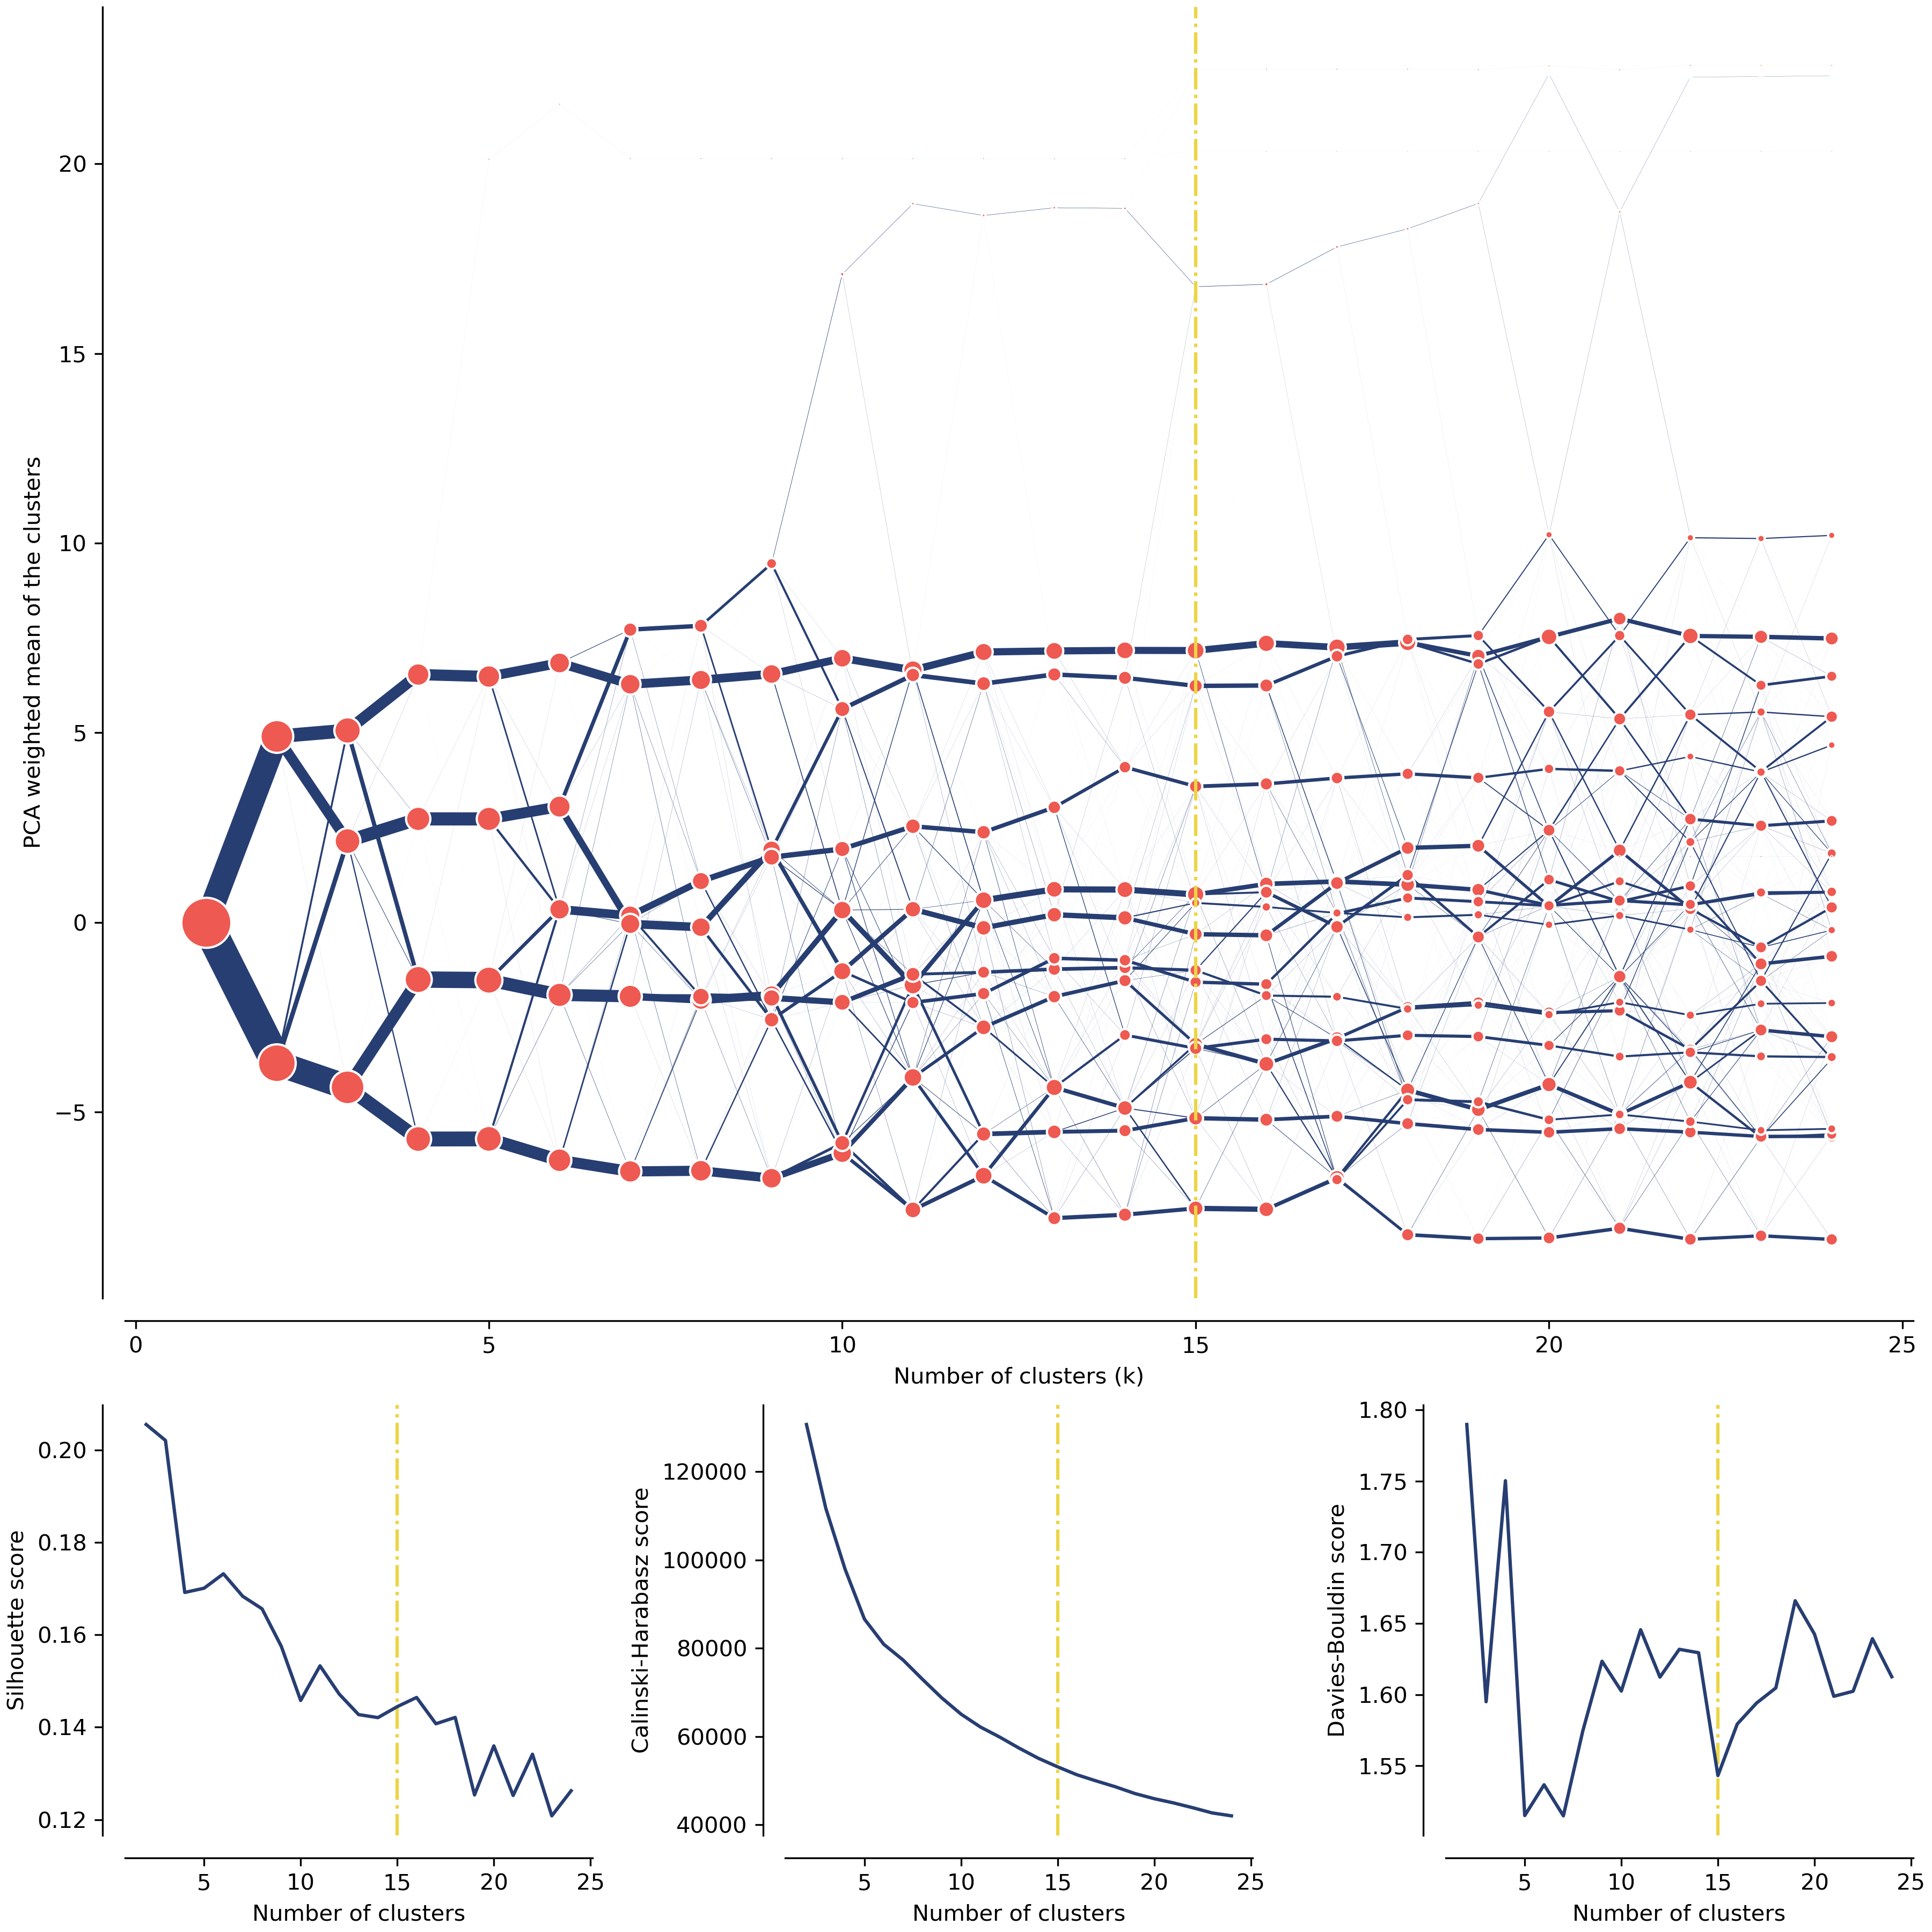
\includegraphics[width=.8\linewidth]{fig/clustergram.png}
    \caption{Clustergram and relevant metrics of a goodness of fit (Silhouette score, C
    alinski-Harabazs score, Davies-Bouldin score) for tested numbers of clusters. The
    clustergram suggest two potential solutions, the very conservative option of 4
    clusters and 10 clusters selected as an optimal resul (indicated by a vertical yellow line).}
    \label{fig:clustergram}
\end{figure}

        % top level providing a first national classification
        % sub clustering of urban areas
            % selection criteria for to-be-subclustered classes
The results of the clustering capture the first group of a national signature
classification composed of ten clusters. However, since the classified ETCs
cover the entirety of space, from vast
natural open spaces to dense city centres, it may result in only a few classes
representing urban areas. While that is caused by the variable heterogeneity of our
dataset in combination with K-Means clustering, the measured characters have the ability
to further distinguish classes of already identified clusters. As spatial signatures
are focused on the urban environment, we further subdivide those clusters covering
a substantial portion of urban areas using another iteration of K-Means clustering
(one class into nine and another into three clusters). Both subdivisions were created using
standard K-Means (single batch) using 1,000 initialisations.
The resulting classification then provide classification capturing the typology of
spatial signatures with a detailed focus on urban development.


% generation of signature geometry
    % dissolution based on contiguity and assigned class
Finally, individual spatial signature geometries are generated as a combination of
adjacent ETCs belonging to the same signature class. To describe each geometry and
each signature type, we measure mean values of the original, non-contextualised
characters, and release it as additional descriptive tables. The resulting numerical
profile of each signature type is available as table \ref{tab:port}. Table \ref{tab:pens} contains pen portraits
derived from these numerical profiles.

\begin{table}
    \begin{tabular}{lrrrrrrrrrrrrrrrr}
        \toprule
        type &  Accessible suburbia &  Connected residential neighbourhoods &  Countryside agriculture &  Dense residential neighbourhoods &  Dense urban neighbourhoods &  Disconnected suburbia &  Concentrated urbanity &  Gridded residential quarters &  Hyper concentrated urbanity &  Local urbanity &  Metropolitan urbanity &  Open sprawl &  Regional urbanity &  Urban buffer &  Warehouse/Park land &  Wild countryside \\
        \midrule
        area of building                                                                                    &               176.95 &                                272.52 &                   204.10 &                            375.60 &                      588.36 &                 212.71 &                3713.38 &                        283.89 &                      3358.10 &          823.35 &                2413.94 &       226.72 &            1480.26 &        209.42 &               393.22 &            209.86 \\
        perimeter of building                                                                               &                53.90 &                                 69.12 &                    56.05 &                             80.56 &                      107.36 &                  61.63 &                 376.30 &                         69.67 &                       330.82 &          135.54 &                 283.94 &        59.64 &             195.98 &         55.94 &                75.68 &             57.12 \\
        courtyard area of building                                                                          &                 0.48 &                                  1.07 &                     0.51 &                              2.13 &                        5.03 &                   0.52 &                 159.09 &                          0.75 &                        90.82 &           12.67 &                 118.95 &         0.90 &              43.19 &          0.74 &                 3.26 &              0.22 \\
        circular compactness of building                                                                    &                 0.53 &                                  0.48 &                     0.51 &                              0.47 &                        0.44 &                   0.49 &                   0.43 &                          0.49 &                         0.45 &            0.41 &                   0.40 &         0.52 &               0.39 &          0.52 &                 0.47 &              0.50 \\
        corners of building                                                                                 &                 4.25 &                                  4.45 &                     4.37 &                              4.69 &                        5.21 &                   4.35 &                  12.48 &                          4.51 &                         9.27 &            6.01 &                   9.72 &         4.37 &               7.78 &          4.34 &                 4.56 &              4.38 \\
        squareness of building                                                                              &                 0.78 &                                  1.47 &                     0.81 &                              1.86 &                        3.28 &                   1.02 &                  18.59 &                          1.66 &                        22.51 &            5.07 &                  12.41 &         0.99 &               8.84 &          0.86 &                 1.35 &              0.71 \\
        equivalent rectangular index of building                                                            &                 0.99 &                                  0.98 &                     0.98 &                              0.97 &                        0.95 &                   0.98 &                   0.78 &                          0.98 &                         0.80 &            0.92 &                   0.82 &         0.98 &               0.87 &          0.98 &                 0.98 &              0.98 \\
        elongation of building                                                                              &                 0.64 &                                  0.56 &                     0.60 &                              0.56 &                        0.52 &                   0.57 &                   0.59 &                          0.58 &                         0.62 &            0.51 &                   0.53 &         0.62 &               0.51 &          0.63 &                 0.54 &              0.59 \\
        centroid - corner mean distance of building                                                         &                 9.60 &                                 12.41 &                     9.79 &                             13.96 &                       18.00 &                  11.11 &                  35.93 &                         12.41 &                        37.22 &           20.71 &                  29.68 &        10.49 &              25.25 &          9.81 &                13.20 &              9.95 \\
        centroid - corner distance deviation of building                                                    &                 0.36 &                                  0.71 &                     0.56 &                              1.07 &                        1.88 &                   0.54 &                   9.03 &                          0.80 &                         7.70 &            2.98 &                   6.78 &         0.55 &               4.98 &          0.49 &                 0.88 &              0.60 \\
        orientation of building                                                                             &                19.56 &                                 25.50 &                    20.57 &                             16.41 &                       20.64 &                  26.39 &                  20.32 &                         23.13 &                        26.26 &           20.78 &                  22.30 &        20.21 &              21.82 &         21.10 &                23.30 &             21.86 \\
        longest axis length of ETC                                                                          &                50.84 &                                 57.72 &                   220.30 &                             64.46 &                       73.56 &                  53.55 &                 112.12 &                         52.89 &                       126.58 &           80.14 &                 100.52 &        60.97 &              91.91 &        105.16 &                78.67 &            449.71 \\
        area of ETC                                                                                         &              1147.25 &                               1517.81 &                 31193.48 &                           1917.31 &                     2410.32 &                1259.03 &                5708.23 &                       1251.54 &                      8654.32 &         2696.40 &                4442.21 &      2000.37 &            3535.28 &       8658.83 &              3520.84 &         155623.92 \\
        circular compactness of ETC                                                                         &                 0.47 &                                  0.48 &                     0.38 &                              0.48 &                        0.47 &                   0.49 &                   0.46 &                          0.48 &                         0.47 &            0.46 &                   0.42 &         0.47 &               0.44 &          0.44 &                 0.46 &              0.35 \\
        equivalent rectangular index of ETC                                                                 &                 0.97 &                                  0.97 &                     0.93 &                              0.96 &                        0.96 &                   0.97 &                   0.94 &                          0.97 &                         0.95 &            0.95 &                   0.93 &         0.97 &               0.94 &          0.95 &                 0.96 &              0.91 \\
        orientation of ETC                                                                                  &                20.40 &                                 24.94 &                    21.92 &                             17.77 &                       21.07 &                  25.28 &                  20.37 &                         23.06 &                        25.96 &           21.22 &                  22.38 &        21.07 &              21.88 &         21.86 &                23.27 &             22.51 \\
        covered area ratio of ETC                                                                           &                 0.19 &                                  0.20 &                     0.07 &                              0.52 &                        0.27 &                   0.22 &                   0.91 &                          0.23 &                         0.61 &            0.60 &                   4.85 &         0.18 &            1122.51 &          0.14 &                 0.18 &              0.04 \\
        cell alignment of building                                                                          &                 7.38 &                                  6.12 &                    11.49 &                              6.52 &                        5.61 &                   8.08 &                   4.43 &                          5.48 &                         2.72 &            5.64 &                   4.86 &         8.64 &               5.25 &          9.76 &                 8.03 &             12.55 \\
        alignment of neighbouring buildings                                                                 &                 5.31 &                                  5.36 &                     8.45 &                              5.39 &                        5.17 &                   5.67 &                   5.95 &                          4.93 &                         6.55 &            5.67 &                   6.37 &         6.48 &               6.27 &          7.06 &                 6.06 &             10.05 \\
        mean distance between neighbouring buildings                                                        &                17.82 &                                 19.17 &                   111.38 &                             20.84 &                       21.13 &                  18.63 &                  18.96 &                         16.48 &                        22.95 &           20.62 &                  22.33 &        22.13 &              20.94 &         45.37 &                28.71 &            238.45 \\
        perimeter-weighted neighbours of ETC                                                                &                 0.04 &                                  0.04 &                     0.02 &                              0.04 &                        0.07 &                   0.05 &                   0.03 &                          0.04 &                         0.04 &            0.11 &                   0.04 &         0.06 &               7.46 &          0.13 &                 0.04 &              0.01 \\
        area covered by neighbouring cells                                                                  &              8620.11 &                              11990.46 &                277883.95 &                          15619.36 &                    20375.37 &                9503.57 &               52023.10 &                       9962.17 &                     61122.40 &        22892.04 &               39665.51 &     16780.98 &           31594.99 &      76942.43 &             31956.96 &        1485709.28 \\
        weighted reached enclosures of ETC                                                                  &                 0.00 &                                  0.00 &                     0.00 &                              0.00 &                        0.00 &                   0.00 &                   0.00 &                          0.00 &                         0.00 &            0.00 &                   0.00 &         0.00 &               0.00 &          0.00 &                 0.00 &              0.00 \\
        mean inter-building distance                                                                        &                21.97 &                                 24.07 &                   167.60 &                             26.48 &                       27.37 &                  22.03 &                  22.73 &                         21.34 &                        23.74 &           26.28 &                  26.99 &        28.94 &              26.32 &         67.27 &                40.97 &            367.72 \\
        width of street profile                                                                             &                28.38 &                                 26.84 &                    32.84 &                             26.29 &                       24.84 &                  27.65 &                  19.47 &                         24.27 &                        17.47 &           24.56 &                  22.61 &        28.59 &              23.44 &         31.00 &                30.85 &             34.31 \\
        width deviation of street profile                                                                   &                 3.30 &                                  3.27 &                     3.91 &                              3.50 &                        3.45 &                   3.71 &                   3.29 &                          3.87 &                         2.85 &            3.60 &                   3.50 &         3.74 &               3.62 &          3.76 &                 3.26 &              3.41 \\
        openness of street profile                                                                          &                 0.42 &                                  0.41 &                     0.83 &                              0.43 &                        0.41 &                   0.44 &                   0.28 &                          0.38 &                         0.22 &            0.41 &                   0.37 &         0.48 &               0.39 &          0.62 &                 0.53 &              0.92 \\
        length of street segment                                                                            &               187.61 &                                162.45 &                   574.25 &                            153.66 &                      151.58 &                 150.53 &                 108.90 &                        126.02 &                        93.90 &          143.14 &                 123.30 &       183.43 &             132.18 &        333.77 &               220.94 &            842.79 \\
        linearity of street segment                                                                         &                 0.93 &                                  0.94 &                     0.93 &                              0.92 &                        0.93 &                   0.92 &                   0.94 &                          0.94 &                         0.97 &            0.92 &                   0.93 &         0.90 &               0.92 &          0.91 &                 0.91 &              0.91 \\
        mean segment length within 3 steps                                                                  &              2327.31 &                               2374.39 &                  5884.25 &                           1992.44 &                     2113.58 &                1707.52 &                1944.94 &                       1950.07 &                      2057.70 &         2011.42 &                2112.12 &      1862.02 &            2034.72 &       3170.78 &              2339.74 &           8062.03 \\
        node degree of junction                                                                             &                 2.87 &                                  3.00 &                     2.78 &                              2.89 &                        2.94 &                   2.68 &                   3.12 &                          3.04 &                         3.33 &            2.94 &                   3.14 &         2.68 &               3.01 &          2.70 &                 2.77 &              2.69 \\
        local meshedness of street network                                                                  &                 0.08 &                                  0.11 &                     0.06 &                              0.10 &                        0.11 &                   0.05 &                   0.14 &                          0.13 &                         0.17 &            0.11 &                   0.14 &         0.06 &               0.12 &          0.05 &                 0.08 &              0.05 \\
        local proportion of 3-way intersections of street network                                           &                 0.74 &                                  0.74 &                     0.72 &                              0.74 &                        0.74 &                   0.71 &                   0.76 &                          0.72 &                         0.70 &            0.75 &                   0.75 &         0.71 &               0.76 &          0.71 &                 0.75 &              0.68 \\
        local proportion of 4-way intersections of street network                                           &                 0.07 &                                  0.12 &                     0.04 &                              0.09 &                        0.11 &                   0.04 &                   0.15 &                          0.16 &                         0.23 &            0.11 &                   0.17 &         0.04 &               0.13 &          0.04 &                 0.05 &              0.04 \\
        local proportion of cul-de-sacs of street network                                                   &                 0.19 &                                  0.14 &                     0.24 &                              0.17 &                        0.14 &                   0.25 &                   0.09 &                          0.12 &                         0.06 &            0.14 &                   0.08 &         0.25 &               0.11 &          0.25 &                 0.20 &              0.28 \\
        local closeness of street network                                                                   &                 0.00 &                                  0.00 &                     0.00 &                              0.00 &                        0.00 &                   0.00 &                   0.00 &                          0.00 &                         0.00 &            0.00 &                   0.00 &         0.00 &               0.00 &          0.00 &                 0.00 &              0.00 \\
        local cul-de-sac length of street network                                                           &               228.58 &                                163.78 &                   636.07 &                            196.63 &                      170.89 &                 275.96 &                  84.41 &                        133.13 &                        75.11 &          167.72 &                  79.56 &       288.26 &             128.76 &        408.67 &               253.49 &           1186.52 \\
        square clustering of street network                                                                 &                 0.03 &                                  0.04 &                     0.01 &                              0.03 &                        0.04 &                   0.01 &                   0.03 &                          0.04 &                         0.04 &            0.03 &                   0.04 &         0.02 &               0.03 &          0.02 &                 0.03 &              0.01 \\
        mean distance to neighbouring nodes of street network                                               &               132.49 &                                118.06 &                   373.74 &                            112.48 &                      111.55 &                 111.69 &                  86.38 &                         92.19 &                        81.24 &          106.90 &                  93.66 &       129.03 &              99.79 &        212.34 &               150.43 &            601.60 \\
        local node density of street network                                                                &                 0.02 &                                  0.02 &                     0.01 &                              0.02 &                        0.02 &                   0.03 &                   0.02 &                          0.02 &                         0.02 &            0.02 &                   0.02 &         0.03 &               0.02 &          0.02 &                 0.02 &              0.01 \\
        local degree weighted node density of street network                                                &                 0.03 &                                  0.03 &                     0.02 &                              0.04 &                        0.04 &                   0.04 &                   0.04 &                          0.04 &                         0.04 &            0.04 &                   0.04 &         0.04 &               0.04 &          0.03 &                 0.03 &              0.01 \\
        street alignment of building                                                                        &                 8.73 &                                  7.53 &                    11.81 &                              8.25 &                        7.57 &                   9.98 &                   7.84 &                          6.95 &                         6.23 &            8.05 &                   8.32 &        10.97 &               8.06 &         11.33 &                10.02 &             12.77 \\
        area covered by node-attached ETCs                                                                  &             22426.36 &                              14599.22 &                286081.33 &                          14037.94 &                    13513.86 &               15656.96 &               13069.71 &                       9488.11 &                     20051.57 &        11878.66 &               13201.87 &     25443.99 &           12080.93 &     100470.30 &             33097.00 &        1215083.95 \\
        area covered by edge-attached ETCs                                                                  &             36496.96 &                              24423.69 &                502883.47 &                          25413.44 &                    26111.44 &               26810.65 &               33257.27 &                      17094.77 &                     38566.99 &        25905.75 &               31497.77 &     47178.87 &           29440.27 &     188719.66 &             66614.68 &        2174736.93 \\
        buildings per meter of street segment                                                               &                 0.11 &                                  0.08 &                     0.05 &                              0.08 &                        0.07 &                   0.10 &                   0.05 &                          0.09 &                         0.05 &            0.06 &                   0.05 &         0.10 &               0.05 &          0.09 &                 0.07 &              0.02 \\
        reached ETCs by neighbouring segments                                                               &                49.09 &                                 33.99 &                    38.08 &                             26.79 &                       21.56 &                  32.35 &                   8.88 &                         26.76 &                         8.57 &           16.97 &                  11.04 &        35.17 &              13.53 &         43.96 &                30.27 &             26.08 \\
        reached area by neighbouring segments                                                               &            113290.06 &                              88462.74 &               1591397.39 &                          89313.79 &                    97515.74 &               84060.33 &              145420.68 &                      64059.40 &                    151507.35 &       100616.06 &              132683.99 &    140813.94 &          119718.73 &     556190.10 &            211678.46 &        5556960.68 \\
        reached ETCs by local street network                                                                &               166.98 &                                126.07 &                   110.89 &                             90.93 &                       74.36 &                 102.39 &                  28.79 &                         99.87 &                        27.00 &           56.17 &                  36.29 &       103.45 &              43.97 &        123.39 &                93.33 &             71.94 \\
        reached area by local street network                                                                &            451276.21 &                             390719.33 &               5858316.88 &                         369240.03 &                   416784.68 &              316062.25 &              703631.50 &                     296524.52 &                    621126.10 &       439804.09 &              643746.00 &    506987.49 &          540975.07 &    1982158.35 &            794621.33 &       17403052.98 \\
        reached ETCs by tessellation contiguity                                                             &                36.80 &                                 40.24 &                    46.23 &                             43.10 &                       45.61 &                  39.57 &                  53.52 &                         42.04 &                        48.46 &           47.29 &                  51.81 &        41.55 &              51.95 &         43.57 &                42.93 &             47.56 \\
        reached area by tessellation contiguity                                                             &             60511.46 &                              87537.63 &               2410926.40 &                         115962.63 &                   152810.21 &               63671.98 &              372984.21 &                      73335.07 &                    306427.88 &       173857.48 &              302746.84 &    136577.35 &          238390.55 &     692699.47 &            297667.66 &       14081627.81 \\
        area of enclosure                                                                                   &            242778.35 &                              95677.02 &               3591565.15 &                         133719.21 &                   105561.74 &              282930.77 &               28859.85 &                     110195.65 &                     31788.41 &        83656.67 &               29460.25 &    640071.17 &           63476.79 &    1854684.23 &            430998.35 &       44036373.80 \\
        perimeter of enclosure                                                                              &              2046.29 &                               1360.81 &                  7599.46 &                           1693.62 &                     1463.16 &                2380.50 &                 683.27 &                       1150.58 &                       538.87 &         1299.32 &                 671.29 &      3793.33 &            1009.07 &       5664.05 &              2992.30 &          21952.84 \\
        circular compactness of enclosure                                                                   &                 0.40 &                                  0.39 &                     0.40 &                              0.38 &                        0.38 &                   0.42 &                   0.44 &                          0.41 &                         0.45 &            0.39 &                   0.40 &         0.38 &               0.40 &          0.39 &                 0.38 &              0.38 \\
        equivalent rectangular index of enclosure                                                           &                 0.85 &                                  0.87 &                     0.84 &                              0.84 &                        0.86 &                   0.83 &                   0.91 &                          0.89 &                         0.94 &            0.85 &                   0.89 &         0.77 &               0.87 &          0.80 &                 0.80 &              0.79 \\
        compactness-weighted axis of enclosure                                                              &               515.77 &                                344.74 &                  1777.66 &                            441.16 &                      397.37 &                 567.78 &                 144.75 &                        289.81 &                       120.13 &          345.64 &                 153.64 &       986.37 &             249.05 &       1434.02 &               780.52 &           5069.06 \\
        orientation of enclosure                                                                            &                19.24 &                                 25.62 &                    21.39 &                             16.18 &                       20.88 &                  27.07 &                  20.23 &                         23.04 &                        24.93 &           21.09 &                  21.77 &        20.39 &              22.00 &         21.52 &                24.08 &             22.66 \\
        perimeter-weighted neighbours of enclosure                                                          &                 0.01 &                                  0.01 &                     0.01 &                              0.02 &                        0.08 &                   0.02 &                   0.04 &                          0.02 &                         0.08 &            0.12 &                   0.06 &         0.05 &               9.94 &          0.11 &                 0.01 &              0.01 \\
        area-weighted ETCs of enclosure                                                                     &                36.32 &                                  2.82 &                   746.28 &                              3.03 &                        4.63 &             2137242.86 &                   0.00 &                          0.43 &                         0.00 &            0.14 &                   0.01 &    330422.61 &               0.01 & 1178106554.77 &            627879.43 &        2270509.66 \\
        Population                                                                                          &                 4.51 &                                  8.57 &                     1.91 &                             10.02 &                       17.52 &                   6.55 &                  36.91 &                          7.74 &                        37.93 &           28.87 &                  43.70 &         5.06 &              42.99 &          3.43 &                 6.93 &              1.31 \\
        Night lights                                                                                        &                11.02 &                                 19.99 &                     1.39 &                             22.63 &                       34.74 &                  12.35 &                 115.70 &                         15.17 &                       183.23 &           51.19 &                  87.38 &        10.96 &              67.53 &          5.08 &                18.29 &              0.48 \\
        Workplace population [Agriculture, energy and water]                                                &                 0.01 &                                  0.03 &                     0.08 &                              0.07 &                        0.11 &                   0.02 &                   2.44 &                          0.03 &                         1.41 &            0.18 &                   1.01 &         0.04 &               0.39 &          0.05 &                 0.10 &              0.11 \\
        Workplace population [Manufacturing]                                                                &                 0.12 &                                  0.29 &                     0.22 &                              0.64 &                        1.10 &                   0.21 &                  12.80 &                          0.36 &                        20.14 &            1.32 &                   4.18 &         0.42 &               2.03 &          0.38 &                 1.25 &              0.09 \\
        Workplace population [Construction]                                                                 &                 0.12 &                                  0.22 &                     0.10 &                              0.33 &                        0.56 &                   0.18 &                   9.16 &                          0.20 &                        10.68 &            0.80 &                   3.80 &         0.17 &               1.40 &          0.14 &                 0.34 &              0.07 \\
        Workplace population [Distribution, hotels and restaurants]                                         &                 0.21 &                                  0.61 &                     0.19 &                              1.17 &                        2.30 &                   0.38 &                  54.16 &                          0.73 &                       152.31 &            4.16 &                  22.76 &         0.45 &              11.90 &          0.32 &                 1.00 &              0.12 \\
        Workplace population [Transport and communication]                                                  &                 0.07 &                                  0.21 &                     0.07 &                              0.41 &                        0.88 &                   0.13 &                  39.51 &                          0.18 &                        97.90 &            1.96 &                  18.93 &         0.16 &               5.70 &          0.14 &                 0.51 &              0.04 \\
        Workplace population [Financial, real estate, professional and administrative activities]           &                 0.15 &                                  0.40 &                     0.13 &                              0.78 &                        1.81 &                   0.26 &                 258.67 &                          0.38 &                       172.75 &            4.89 &                  65.30 &         0.27 &              16.45 &          0.21 &                 0.61 &              0.06 \\
        Workplace population [Public administration, education and health]                                  &                 0.43 &                                  0.94 &                     0.22 &                              1.67 &                        3.21 &                   0.59 &                  41.70 &                          0.98 &                        30.82 &            5.71 &                  42.90 &         0.59 &              14.50 &          0.39 &                 1.06 &              0.12 \\
        Workplace population [Other]                                                                        &                 0.06 &                                  0.15 &                     0.05 &                              0.26 &                        0.56 &                   0.10 &                  23.06 &                          0.17 &                        38.16 &            1.14 &                   8.74 &         0.09 &               3.40 &          0.07 &                 0.16 &              0.03 \\
        Land cover [Airports]                                                                               &                 0.00 &                                  0.00 &                     0.00 &                              0.00 &                        0.00 &                   0.00 &                   0.00 &                          0.00 &                         0.00 &            0.00 &                   0.00 &         0.00 &               0.00 &          0.00 &                 0.00 &              0.00 \\
        Land cover [Non-irrigated arable land]                                                              &                 0.00 &                                  0.00 &                     0.35 &                              0.00 &                        0.00 &                   0.00 &                   0.00 &                          0.00 &                         0.00 &            0.00 &                   0.00 &         0.01 &               0.00 &          0.11 &                 0.02 &              0.15 \\
        Land cover [Industrial or commercial units]                                                         &                 0.00 &                                  0.02 &                     0.01 &                              0.05 &                        0.09 &                   0.01 &                   0.00 &                          0.00 &                         0.00 &            0.09 &                   0.01 &         0.03 &               0.06 &          0.03 &                 0.14 &              0.00 \\
        Land cover [Salt marshes]                                                                           &                 0.00 &                                  0.00 &                     0.00 &                              0.00 &                        0.00 &                   0.00 &                   0.00 &                          0.00 &                         0.01 &            0.00 &                   0.00 &         0.00 &               0.00 &          0.00 &                 0.00 &              0.00 \\
        Land cover [Estuaries]                                                                              &                 0.00 &                                  0.00 &                     0.00 &                              0.00 &                        0.00 &                   0.00 &                   0.00 &                          0.00 &                         0.00 &            0.00 &                   0.00 &         0.00 &               0.00 &          0.00 &                 0.00 &              0.00 \\
        Land cover [Sport and leisure facilities]                                                           &                 0.00 &                                  0.00 &                     0.02 &                              0.00 &                        0.00 &                   0.00 &                   0.00 &                          0.00 &                         0.00 &            0.00 &                   0.00 &         0.01 &               0.00 &          0.02 &                 0.01 &              0.01 \\
        Land cover [Green urban areas]                                                                      &                 0.01 &                                  0.01 &                     0.00 &                              0.01 &                        0.01 &                   0.00 &                   0.03 &                          0.00 &                         0.00 &            0.01 &                   0.03 &         0.01 &               0.01 &          0.00 &                 0.02 &              0.00 \\
        Land cover [Discontinuous urban fabric]                                                             &                 0.98 &                                  0.95 &                     0.20 &                              0.88 &                        0.75 &                   0.98 &                   0.06 &                          0.92 &                         0.00 &            0.63 &                   0.08 &         0.91 &               0.34 &          0.68 &                 0.77 &              0.03 \\
        Land cover [Pastures]                                                                               &                 0.00 &                                  0.00 &                     0.36 &                              0.00 &                        0.00 &                   0.00 &                   0.00 &                          0.00 &                         0.02 &            0.00 &                   0.00 &         0.02 &               0.00 &          0.12 &                 0.02 &              0.59 \\
        Land cover [Broad-leaved forest]                                                                    &                 0.00 &                                  0.00 &                     0.02 &                              0.00 &                        0.00 &                   0.00 &                   0.00 &                          0.00 &                         0.00 &            0.00 &                   0.00 &         0.00 &               0.00 &          0.01 &                 0.00 &              0.03 \\
        Land cover [Mineral extraction sites]                                                               &                 0.00 &                                  0.00 &                     0.00 &                              0.00 &                        0.00 &                   0.00 &                   0.00 &                          0.00 &                         0.00 &            0.00 &                   0.00 &         0.00 &               0.00 &          0.00 &                 0.00 &              0.00 \\
        Land cover [Port areas]                                                                             &                 0.00 &                                  0.00 &                     0.00 &                              0.00 &                        0.01 &                   0.00 &                   0.00 &                          0.00 &                         0.00 &            0.01 &                   0.00 &         0.00 &               0.01 &          0.00 &                 0.01 &              0.00 \\
        Land cover [Road and rail networks and associated land]                                             &                 0.00 &                                  0.00 &                     0.00 &                              0.00 &                        0.00 &                   0.00 &                   0.00 &                          0.00 &                         0.00 &            0.00 &                   0.00 &         0.00 &               0.00 &          0.00 &                 0.00 &              0.00 \\
        Land cover [Water bodies]                                                                           &                 0.00 &                                  0.00 &                     0.00 &                              0.00 &                        0.00 &                   0.00 &                   0.00 &                          0.00 &                         0.00 &            0.00 &                   0.00 &         0.00 &               0.00 &          0.00 &                 0.00 &              0.00 \\
        Land cover [Land principally occupied by agriculture, with significant areas of natural vegetation] &                 0.00 &                                  0.00 &                     0.01 &                              0.00 &                        0.00 &                   0.00 &                   0.00 &                          0.00 &                         0.00 &            0.00 &                   0.00 &         0.00 &               0.00 &          0.00 &                 0.00 &              0.01 \\
        Land cover [Mixed forest]                                                                           &                 0.00 &                                  0.00 &                     0.01 &                              0.00 &                        0.00 &                   0.00 &                   0.00 &                          0.00 &                         0.00 &            0.00 &                   0.00 &         0.00 &               0.00 &          0.00 &                 0.00 &              0.02 \\
        Land cover [Peat bogs]                                                                              &                 0.00 &                                  0.00 &                     0.00 &                              0.00 &                        0.00 &                   0.00 &                   0.00 &                          0.00 &                         0.00 &            0.00 &                   0.00 &         0.00 &               0.00 &          0.00 &                 0.00 &              0.02 \\
        Land cover [Natural grasslands]                                                                     &                 0.00 &                                  0.00 &                     0.00 &                              0.00 &                        0.00 &                   0.00 &                   0.00 &                          0.00 &                         0.00 &            0.00 &                   0.00 &         0.00 &               0.00 &          0.00 &                 0.00 &              0.04 \\
        Land cover [Moors and heathland]                                                                    &                 0.00 &                                  0.00 &                     0.00 &                              0.00 &                        0.00 &                   0.00 &                   0.00 &                          0.00 &                         0.00 &            0.00 &                   0.00 &         0.00 &               0.00 &          0.00 &                 0.00 &              0.04 \\
        Land cover [Transitional woodland-shrub]                                                            &                 0.00 &                                  0.00 &                     0.00 &                              0.00 &                        0.00 &                   0.00 &                   0.00 &                          0.00 &                         0.00 &            0.00 &                   0.00 &         0.00 &               0.00 &          0.00 &                 0.00 &              0.01 \\
        Land cover [Continuous urban fabric]                                                                &                 0.00 &                                  0.02 &                     0.00 &                              0.04 &                        0.13 &                   0.00 &                   0.90 &                          0.07 &                         0.97 &            0.25 &                   0.88 &         0.00 &               0.57 &          0.00 &                 0.00 &              0.00 \\
        Land cover [Intertidal flats]                                                                       &                 0.00 &                                  0.00 &                     0.00 &                              0.00 &                        0.00 &                   0.00 &                   0.00 &                          0.00 &                         0.00 &            0.00 &                   0.00 &         0.00 &               0.00 &          0.00 &                 0.00 &              0.00 \\
        Land cover [Sea and ocean]                                                                          &                 0.00 &                                  0.00 &                     0.00 &                              0.00 &                        0.00 &                   0.00 &                   0.00 &                          0.00 &                         0.00 &            0.00 &                   0.00 &         0.00 &               0.00 &          0.00 &                 0.00 &              0.00 \\
        Land cover [Construction sites]                                                                     &                 0.00 &                                  0.00 &                     0.00 &                              0.00 &                        0.00 &                   0.00 &                   0.00 &                          0.00 &                         0.00 &            0.00 &                   0.00 &         0.00 &               0.00 &          0.01 &                 0.00 &              0.00 \\
        Land cover [Burnt areas]                                                                            &                 0.00 &                                  0.00 &                     0.00 &                              0.00 &                        0.00 &                   0.00 &                   0.00 &                          0.00 &                         0.00 &            0.00 &                   0.00 &         0.00 &               0.00 &          0.00 &                 0.00 &              0.00 \\
        Land cover [Dump sites]                                                                             &                 0.00 &                                  0.00 &                     0.00 &                              0.00 &                        0.00 &                   0.00 &                   0.00 &                          0.00 &                         0.00 &            0.00 &                   0.00 &         0.00 &               0.00 &          0.00 &                 0.00 &              0.00 \\
        Land cover [Complex cultivation patterns]                                                           &                 0.00 &                                  0.00 &                     0.00 &                              0.00 &                        0.00 &                   0.00 &                   0.00 &                          0.00 &                         0.00 &            0.00 &                   0.00 &         0.00 &               0.00 &          0.00 &                 0.00 &              0.00 \\
        Land cover [Inland marshes]                                                                         &                 0.00 &                                  0.00 &                     0.00 &                              0.00 &                        0.00 &                   0.00 &                   0.00 &                          0.00 &                         0.00 &            0.00 &                   0.00 &         0.00 &               0.00 &          0.00 &                 0.00 &              0.00 \\
        Land cover [Water courses]                                                                          &                 0.00 &                                  0.00 &                     0.00 &                              0.00 &                        0.00 &                   0.00 &                   0.01 &                          0.00 &                         0.00 &            0.00 &                   0.01 &         0.00 &               0.01 &          0.00 &                 0.00 &              0.00 \\
        Land cover [Coniferous forest]                                                                      &                 0.00 &                                  0.00 &                     0.01 &                              0.00 &                        0.00 &                   0.00 &                   0.00 &                          0.00 &                         0.00 &            0.00 &                   0.00 &         0.00 &               0.00 &          0.00 &                 0.00 &              0.04 \\
        Land cover [Bare rocks]                                                                             &                 0.00 &                                  0.00 &                     0.00 &                              0.00 &                        0.00 &                   0.00 &                   0.00 &                          0.00 &                         0.00 &            0.00 &                   0.00 &         0.00 &               0.00 &          0.00 &                 0.00 &              0.00 \\
        Land cover [Coastal lagoons]                                                                        &                 0.00 &                                  0.00 &                     0.00 &                              0.00 &                        0.00 &                   0.00 &                   0.00 &                          0.00 &                         0.00 &            0.00 &                   0.00 &         0.00 &               0.00 &          0.00 &                 0.00 &              0.00 \\
        Land cover [Beaches, dunes, sands]                                                                  &                 0.00 &                                  0.00 &                     0.00 &                              0.00 &                        0.00 &                   0.00 &                   0.00 &                          0.00 &                         0.00 &            0.00 &                   0.00 &         0.00 &               0.00 &          0.00 &                 0.00 &              0.00 \\
        Land cover [Agro-forestry areas]                                                                    &                 0.00 &                                  0.00 &                     0.00 &                              0.00 &                        0.00 &                   0.00 &                   0.00 &                          0.00 &                         0.00 &            0.00 &                   0.00 &         0.00 &               0.00 &          0.00 &                 0.00 &              0.00 \\
        Land cover [Sparsely vegetated areas]                                                               &                 0.00 &                                  0.00 &                     0.00 &                              0.00 &                        0.00 &                   0.00 &                   0.00 &                          0.00 &                         0.00 &            0.00 &                   0.00 &         0.00 &               0.00 &          0.00 &                 0.00 &              0.00 \\
        Land cover [Fruit trees and berry plantations]                                                      &                 0.00 &                                  0.00 &                     0.00 &                              0.00 &                        0.00 &                   0.00 &                   0.00 &                          0.00 &                         0.00 &            0.00 &                   0.00 &         0.00 &               0.00 &          0.00 &                 0.00 &              0.00 \\
        NDVI                                                                                                &                 0.29 &                                  0.25 &                     0.48 &                              0.23 &                        0.19 &                   0.29 &                   0.03 &                          0.21 &                         0.00 &            0.16 &                   0.06 &         0.29 &               0.11 &          0.37 &                 0.29 &              0.56 \\
        Supermarkets [distance to nearest]                                                                  &               828.82 &                                679.96 &                  4751.23 &                            661.77 &                      587.28 &                 761.86 &                 229.90 &                        577.68 &                       324.42 &          483.02 &                 299.93 &       948.03 &             331.07 &       1752.87 &              1043.84 &           9854.12 \\
        Supermarkets [counts within 1200m]                                                                  &                 1.89 &                                  2.86 &                     0.09 &                              3.13 &                        4.44 &                   2.07 &                  22.51 &                          3.41 &                        18.79 &            6.85 &                  17.27 &         1.47 &              12.53 &          0.65 &                 1.43 &              0.03 \\
        Listed buildings [distance to nearest]                                                              &               744.22 &                                596.61 &                   557.94 &                            506.61 &                      350.89 &                 729.61 &                  31.73 &                        516.20 &                        69.75 &          216.86 &                  51.87 &       760.26 &             115.00 &        673.93 &               934.00 &           1324.03 \\
        Listed buildings [counts within 1200m]                                                              &                11.27 &                                 24.28 &                    11.22 &                             37.47 &                       62.78 &                  24.18 &                 685.16 &                         31.77 &                      1142.57 &          140.03 &                 456.53 &        18.17 &             324.50 &         16.14 &                10.57 &              4.21 \\
        FHRS points [distance to nearest]                                                                   &               218.46 &                                152.48 &                   725.69 &                            144.02 &                      106.08 &                 217.95 &                  16.22 &                        129.24 &                        14.10 &           82.47 &                  40.06 &       267.24 &              56.87 &        379.17 &               256.22 &           1699.17 \\
        FHRS points [counts within 1200m]                                                                   &               334.43 &                                692.66 &                    44.47 &                            860.93 &                     1568.44 &                 342.08 &                6297.61 &                       1081.38 &                      9213.15 &         2167.91 &                4490.95 &       253.88 &            3163.83 &        132.66 &               271.09 &             33.07 \\
        Cultural venues [distance to nearest]                                                               &              5384.64 &                               3946.05 &                 13156.20 &                           3497.51 &                     2287.43 &                5831.52 &                 702.75 &                       4094.92 &                       351.33 &         1273.23 &                 644.53 &      6309.75 &             850.25 &       8939.65 &              5121.47 &          20695.29 \\
        Cultural venues [counts within 1200m]                                                               &                 0.06 &                                  0.13 &                     0.00 &                              0.26 &                        0.48 &                   0.08 &                  10.39 &                          0.24 &                        34.20 &            1.13 &                   4.45 &         0.06 &               2.23 &          0.02 &                 0.06 &              0.00 \\
        Water bodies [distance to nearest]                                                                  &               542.61 &                                555.96 &                   304.49 &                            483.12 &                      528.85 &                 523.05 &                 565.25 &                        522.09 &                       759.60 &          507.71 &                 467.71 &       378.36 &             461.42 &        345.79 &               417.43 &            236.73 \\
        Retail centres [distance to nearest]                                                                &               849.45 &                                536.47 &                  4943.97 &                            421.09 &                      224.33 &                 725.57 &                  29.80 &                        445.52 &                        32.54 &          161.85 &                  66.32 &      1002.66 &              90.87 &       2102.46 &               898.17 &          11041.32 \\
        \bottomrule
        \end{tabular}

        \caption{\label{tab:port}Numerical portraits characterising each signature type. Each value is computed as a mean of values of all ETCs within the type.}

    \end{table}


\begin{table}
\begin{tabular}{ll}
    \toprule
    {} &                                                                                                                                                                                                                                                                                                                                                                                                                             0 \\
    \midrule
    Wild countryside                     &                                                                                       In “Wild countryside”, human influence is the least intensive. This signature covers large open spaces in the countryside where no urbanisation happens apart from occasional roads, cottages, and pastures. You can find it across the Scottish Highlands, numerous national parks such as Lake District, or in the majority of Wales. \\
    Countryside agriculture              &                                                                                                                                                                               “Countryside agriculture” features much of the English countryside and displays a high degree of agriculture including both fields and pastures. There are a few buildings scattered across the area but, for the most part, it is green space. \\
    Urban buffer                         &                                                                                             “Urban buffer” can be characterised as a green belt around cities. This signature includes mostly agricultural land in the immediate adjacency of towns and cities, often including edge development. It still feels more like countryside than urban, but these signatures are much smaller compared to other countryside types. \\
    Open sprawl                          &                                                                                                                           “Open sprawl” represents the transition between countryside and urbanised land. It is located in the outskirts of cities or around smaller towns and is typically made up of large open space areas intertwined with different kinds of human development, from highways to smaller neighbourhoods. \\
    Disconnected suburbia                &                                                                                                                                           “Disconnected suburbia” includes residential developments in the outskirts of cities or even towns and villages with convoluted, disconnected street networks, low built-up and population densities, and lack of jobs and services. This signature type is entirely car-dependent. \\
    Accessible suburbia                  &                                        “Accessible suburbia” covers residential development on the urban periphery with a relatively legible and connected street network, albeit less so than other more urban signature types. Areas in this signature feature low density, both in terms of population and built-up area, lack of jobs and services. For these reasons, “accessible suburbia” largely acts as dormitories. \\
    Warehouse/Park land                  &                                “Warehouse/Park land” covers predominantly industrial areas and other work-related developments made of box-like buildings with large footprints. It contains many jobs of manual nature such as manufacturing or construction, and very little population live here compared to the rest of urban areas. Occasionally this type also covers areas of parks with large scale green open areas. \\
    Gridded residential quarters         &                                                                                  “Gridded residential quarters” are areas with street networks forming a well-connected grid-like (high density of 4-way intersections) pattern, resulting in places with smaller blocks and higher granularity. This signature is mostly residential but includes some services and jobs, and it tends to be located away from city centres. \\
    Connected residential neighbourhoods &                                                                     “Connected residential neighbourhoods” are relatively dense urban areas, both in terms of population and built-up area, that tend to be formed around well-connected street networks. They have access to services and some jobs but may be further away from city centres leading to higher dependency on cars and public transport for their residents. \\
    Dense residential neighbourhoods     &                                                                                                                                           A “dense residential neighbourhood” is an abundant signature often covering large parts of cities outside of their centres. It has primarily residential purpose and high population density, varied street network patterns, and some services and jobs but not in high intensity. \\
    Dense urban neighbourhoods           &                                                                                                                            “Dense urban neighbourhoods” are areas of inner-city with high population and built-up density of a predominantly residential nature but with direct access to jobs and services. This signature type tends to be relatively walkable and, in the case of some towns, may even form their centres. \\
    Local urbanity                       &                                                                “Local urbanity” reflects town centres, outer parts of city centres or even district centres. In all cases, this signature is very much urban in essence, combining high population and built-up density, access to amenities and jobs. Yet, it is on the lower end of the hierarchy of signature types denoting urban centres with only a local significance. \\
    Regional urbanity                    &                                                             “Regional urbanity” captures centres of mid-size cities with regional importance such as Liverpool, Plymouth or Newcastle upon Tyne. It is often encircled by “Local urbanity” signatures and can form outer rings of city centres in large cities. It features high population density, as well as a high number of jobs and amenities within walkable distance. \\
    Metropolitan urbanity                &                                                                                    Signature type “Metropolitan urbanity” captures the centre of the largest cities in Great Britain such as Glasgow, Birmingham or Manchester. It is characterised by a very high number of jobs in the area, high built-up density and often high population density. This type serves as the core centre of the entire metropolitan areas. \\
    Concentrated urbanity                &  Concentrated urbanity” is a signature type found in the city centre of London and nowhere else in Great Britain. It reflects the uniqueness of London in the British context with an extremely high number of jobs and amenities located nearby, as well as high built-up and population densities. Buildings in this signature are large and tightly packed, forming complex shapes with courtyards and little green space. \\
    Hyper concentrated urbanity          &     The epitome of urbanity in the British context. “Hyper concentrated urbanity” is a signature type present only in the centre of London, around the Soho district, and covering Oxford and Regent streets. This signature is the result of centuries of urban primacy, with a multitude of historical layers interwoven, very high built-up and population density, and extreme abundance of amenities, services and jobs. \\
    \bottomrule
    \end{tabular}
\caption{\label{tab:pens}Interpretative pen portraits characterising each signature type based on its numerical profile.}
\end{table}
% - Feature importance - should this actually be included in here? It is not part of the
%   data product so I'd say no.
